\chapter{神经科学概述}

\section{BCI 介绍}

由于现代计算机技术和神经科学学科的迅速发展,人们已经可以将大脑中的运动与计算机设备相关联,通过机器捕捉大脑中各个通道的活动(Review见Van Gerven et al., 2009 和Wolpaw et al. 2002)。这种方法与应用统称为脑机接口(brain computer interface,或BCI),以探索大脑活动与特定神经状态的关系。其中特定的神经状态也叫做签名(signatures)。如图\ref{Fig:bci_brief}所示,一个BCI需要包括:
\begin{enumerate}
\item{记录大脑活动}
\item{提取并处理签名}
\item{将签名翻译成计算机指令}
\item{最后返回给用户}
\end{enumerate}

整个过程的技术。

\begin{figure}[htb]
\centering
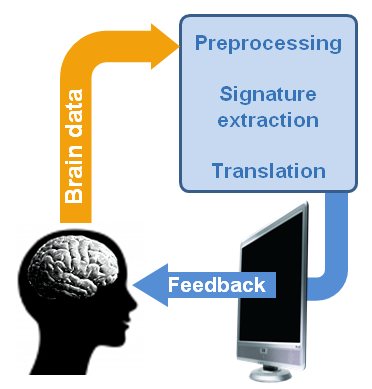
\includegraphics[scale=0.8]{Pictures/Chap1/bci_cycle_v2-2.png}
\caption{BCI 框架}
\label{Fig:bci_brief}
\end{figure}





\section{大脑的概念感知}


猴子对复杂的可视化刺激可以快速反应, 平均反应时间在250-260ms, 最短可以达到180ms。 如图\ref{Fig:brain_stimulate_flow}所示为一个基于视觉刺激, 从视网膜到肌肉执行操作的有可能的大脑通路图\cite{thorpe2001seeking}。 信息从视网膜传递到背外侧膝状体核(lateral geniculate necleus, LGN), 经过延迟传递到V1(主要的视觉皮层) 。 紧接着, 信息经过V2区,V4区,再到后、前颞皮质区(Inferotemporal cortex), 进行物体(高层)特征分析与描述。 后颞皮质将信息映射到不同区域,包括可以进行物体分类的前额皮质(prefrontal cortex cortex, PFC)。 为了将理解的命令传给肌肉执行, PFC又把信息通过运动前皮质区(premotor cortex, PMC)和运动皮层(motor cortex, MC)传递给脊髓的运动神经元。 最后,脊髓的运动神经元受刺激从而触发肌肉运动。 图中, 每个信息处理过程后有一个以毫秒为单位的时间, 表示信息处理的估计时间。


\begin{figure}[htb]
\centering
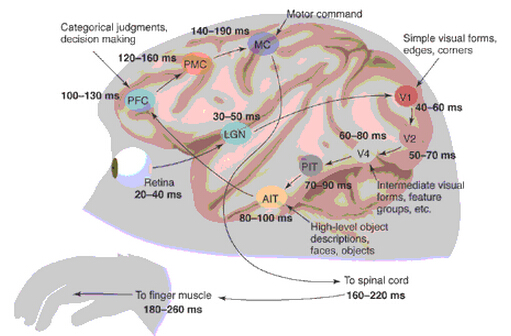
\includegraphics{Pictures/Introduction/brain_flow.jpg}
\caption{可视化刺激任务的大脑通路}
\label{Fig:brain_stimulate_flow}
\end{figure}


\section{P300}\label{sec:introduction_p300}


现在有很多测量脑信号的技术,如fMRI (functional magnetic resonance imaging,功能性磁共振成像),NIRS(near-infrared spectroscopy,近红外光谱学),EEG(Electroencephalograph,脑电图),MEG(Magnetoencephalography,脑磁图)等。针对不同的采集信号,其信号预处理方法也各不相同。但是BCI最基本的任务都是正确地识别“签名”并翻译成机器指令以完成用户的意愿。在P300拼写中,可以通过“oddball task”(如图\ref{Fig:P300_brief})产生P300信号。这个oddball task是一个关于字符注意的实验,展现一串字符(如SSTSSSSTSS),其中出现频率高的称为标准刺激(如该信号序列中的S),频率低的称为异常刺激(如该信号序列中的T)。当出现一个异常刺激时,300ms后就会在EEG信号中产生一个正向偏移。这里标准刺激和异常刺激的差异可以用来识别所给刺激的类别,然后基于刺激发送信号给计算机指令执行。
 
\begin{figure}[htb]
\centering
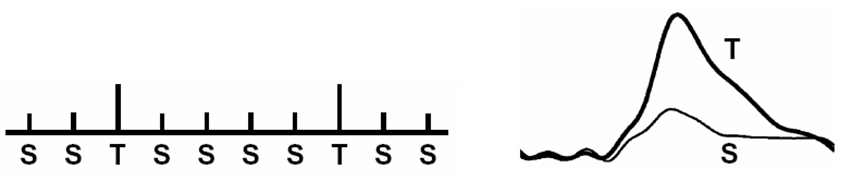
\includegraphics[scale=0.6]{Pictures/Chap1/p300_example.png}
\caption{P300刺激信号}
\label{Fig:P300_brief}
\end{figure}
Figure 2. 标准刺激(S)中的异常刺激(T)

在P300实验中,字母都展现在一个matrix中,其中同一时刻只有一行或一列亮起,具体哪一行或哪一列随机闪现。如下图所示,当一行一列相继闪烁的交点为指定字母时,测试者可以集中精神在头脑中进行简单计数或者确认,相应就会有P300产生。





